%%%%%%%%%%%%%%%%%%%%%%%%%%%%%%%%%%%%%%%%%
% Beamer Presentation
% LaTeX Template
% Version 1.0 (10/11/12)
%
% This template has been downloaded from:
% http://www.LaTeXTemplates.com
%
% License:
% CC BY-NC-SA 3.0 (http://creativecommons.org/licenses/by-nc-sa/3.0/)
%
%%%%%%%%%%%%%%%%%%%%%%%%%%%%%%%%%%%%%%%%%

%----------------------------------------------------------------------------------------
%	PACKAGES AND THEMES
%----------------------------------------------------------------------------------------

\documentclass{beamer}

\mode<presentation> {

% The Beamer class comes with a number of default slide themes
% which change the colors and layouts of slides. Below this is a list
% of all the themes, uncomment each in turn to see what they look like.

%\usetheme{default}
%\usetheme{AnnArbor}
%\usetheme{Antibes}
%\usetheme{Bergen}
%\usetheme{Berkeley}
%\usetheme{Berlin}
%\usetheme{Boadilla}
\usetheme{CambridgeUS}
%\usetheme{Copenhagen}
%\usetheme{Darmstadt}
%\usetheme{Dresden}
%\usetheme{Frankfurt}
%\usetheme{Goettingen}
%\usetheme{Hannover}
%\usetheme{Ilmenau}
%\usetheme{JuanLesPins}
%\usetheme{Luebeck}
%\usetheme{Madrid}
%\usetheme{Malmoe}
%\usetheme{Marburg}
%\usetheme{Montpellier}
%\usetheme{PaloAlto}
%\usetheme{Pittsburgh}
%\usetheme{Rochester}
%\usetheme{Singapore}
%\usetheme{Szeged}
%\usetheme{Warsaw}

% As well as themes, the Beamer class has a number of color themes
% for any slide theme. Uncomment each of these in turn to see how it
% changes the colors of your current slide theme.

%\usecolortheme{albatross}
%\usecolortheme{beaver}
%\usecolortheme{beetle}
%\usecolortheme{crane}
%\usecolortheme{dolphin}
%\usecolortheme{dove}
%\usecolortheme{fly}
%\usecolortheme{lily}
%\usecolortheme{orchid}
%\usecolortheme{rose}
%\usecolortheme{seagull}
%\usecolortheme{seahorse}
%\usecolortheme{whale}
%\usecolortheme{wolverine}

%\setbeamertemplate{footline} % To remove the footer line in all slides uncomment this line
%\setbeamertemplate{footline}[page number] % To replace the footer line in all slides with a simple slide count uncomment this line

%\setbeamertemplate{navigation symbols}{} % To remove the navigation symbols from the bottom of all slides uncomment this line
}

\usepackage{ctex} % 支持中文字体与格式
\usepackage{graphicx} % Allows including images
\usepackage{booktabs} % Allows the use of \toprule, \midrule and \bottomrule in tables


%----------------------------------------------------------------------------------------
%	TITLE PAGE
%----------------------------------------------------------------------------------------

\title[PPT 模板]{Presentation 标题} % The short title appears at the bottom of every slide, the full title is only on the title page

\author{郑启明} % Your name
\institute[SWJTU] % Your institution as it will appear on the bottom of every slide, may be shorthand to save space
{
西南交通大学 \\ % Your institution for the title page
\medskip
\textit{mail@qmz.me} % Your email address
}\setCJKmainfont{SimSun}  
\date{\today} % Date, can be changed to a custom date

\begin{document}

\begin{frame}
\titlepage % Print the title page as the first slide
\end{frame}

\begin{frame}
\frametitle{大纲} % Table of contents slide, comment this block out to remove it
\tableofcontents % Throughout your presentation, if you choose to use \section{} and \subsection{} commands, these will automatically be printed on this slide as an overview of your presentation
\end{frame}

%----------------------------------------------------------------------------------------
%	PRESENTATION SLIDES
%----------------------------------------------------------------------------------------

%------------------------------------------------
\section{普通使用方式} % Sections can be created in order to organize your presentation into discrete blocks, all sections and subsections are automatically printed in the table of contents as an overview of the talk
%------------------------------------------------

\subsection{文字与格式} % A subsection can be created just before a set of slides with a common theme to further break down your presentation into chunks

\begin{frame}
\frametitle{句段}

本人在Github上面布置了一份使用Xelatex编译器生成中文 PPT 的种子。主要作用就是使用Latex 生成实验室做(学术)报告用的演示文稿。\\~\\

Latex用来做学术报告的好处自然不用多说,对于公式、表格、数据、图表的支持都很上道,由于对于已经使用Latex排版完成论文或者实验报告的同学来说更是方便至极。

\end{frame}

%------------------------------------------------

\begin{frame}
\frametitle{无序列表}
\begin{itemize}
\item 盈盈一水间,默默不得语
\item 自在飞花轻似梦
\item 寒来暑往,秋收冬藏
\item 发现更大的世界
\item 倬彼甫田,岁取十千。我取其陈,食我农人。自古有年。今适南亩,或耘或耔。黍稷薿薿,攸介攸止,烝我髦士。
\end{itemize}
\end{frame}

%------------------------------------------------

\begin{frame}
\frametitle{高亮文字框}

\begin{block}{青蝇}
营营青蝇,止于樊。岂弟君子,无信谗言。

营营青蝇,止于棘。谗人罔极,交乱四国。

营营青蝇,止于榛。谗人罔极,构我二人。
\end{block}

\begin{block}{山有扶苏}
山有扶苏,隰有荷华。不见子都,乃见狂且。

山有乔松,隰有游龙,不见子充,乃见狡童。
\end{block}

\end{frame}

%------------------------------------------------

\begin{frame}
\frametitle{多列布局}
\begin{columns}[c] % The "c" option specifies centered vertical alignment while the "t" option is used for top vertical alignment

\column{.45\textwidth} % Left column and width
\textbf{小标题}
\begin{enumerate}
\item 孤藤
\item 老树
\item 昏鸦
\end{enumerate}

\column{.5\textwidth} % Right column and width

风雨凄凄,鸡鸣喈喈,既见君子。云胡不夷?

风雨潇潇,鸡鸣胶胶。既见君子,云胡不瘳?

风雨如晦,鸡鸣不已。既见君子,云胡不喜?

\end{columns}
\end{frame}

%------------------------------------------------
\section{高级用法}
%------------------------------------------------

\begin{frame}
\frametitle{表}
\begin{table}
\begin{tabular}{l l l}
\toprule
\textbf{项目} & \textbf{数据 1} & \textbf{数据 2}\\
\midrule
项目 1 & 0.0003262 & 0.562 \\
项目 2 & 0.0015681 & 0.910 \\
项目 3 & 0.0009271 & 0.296 \\
\bottomrule
\end{tabular}
\caption{表注}
\end{table}
\end{frame}

%------------------------------------------------

\begin{frame}
\frametitle{定理}
\begin{theorem}[质量守恒]
$E = mc^2$
\end{theorem}
\end{frame}

%------------------------------------------------

\begin{frame}[fragile] % Need to use the fragile option when verbatim is used in the slide
\frametitle{代码}
\begin{example}[上页的代码]
\begin{verbatim}
\begin{frame}
\frametitle{Theorem}
\begin{theorem}[Mass--energy equivalence]
$E = mc^2$
\end{theorem}
\end{frame}\end{verbatim}
\end{example}
\end{frame}

%------------------------------------------------

\begin{frame}
\frametitle{图片}
\begin{figure}
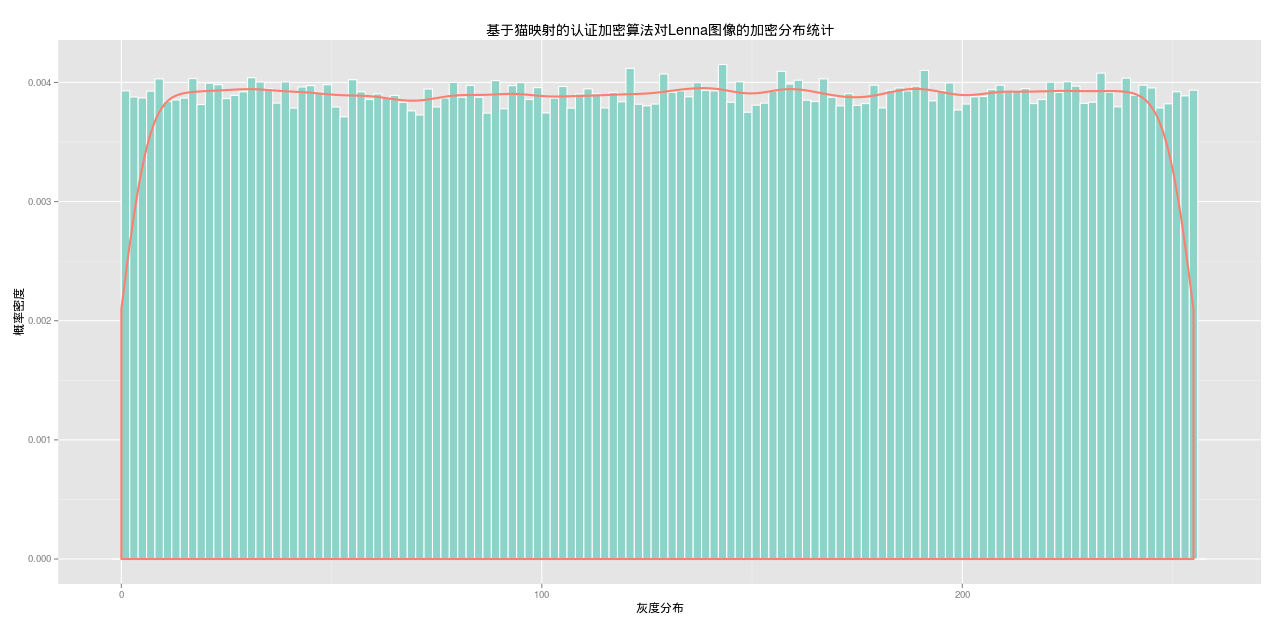
\includegraphics[width=0.8\linewidth]{./images/histogram.png}
\end{figure}
\end{frame}

%------------------------------------------------

\begin{frame}[fragile] % Need to use the fragile option when verbatim is used in the slide
\frametitle{引用}
使用 \verb|\cite| 命令来添加引用\\~

带有引用的文字 \cite{p1}.
\end{frame}

%------------------------------------------------

\begin{frame}
\frametitle{参考文献}
\footnotesize{
\begin{thebibliography}{99} % Beamer does not support BibTeX so references must be inserted manually as below
\bibitem[张三, 2015]{p1} 张三 (2015)
\newblock 文献名称
\newblock \emph{期刊名称} 15(3), 45 -- 678.
\end{thebibliography}
}
\end{frame}

%------------------------------------------------

\begin{frame}
\Huge{\centerline{谢谢}}
\end{frame}

%----------------------------------------------------------------------------------------

\end{document} 